\state{(Jackson 14.4)}{
	Using the {\Lienard}-Wiechart fields, discuss the time-averaged power radiated per unit solid angle in nonrelativistic motion of a particle with charge $e$, moving as described below.  Sketch the angular distribution of the radiation and determine the total power radiated in each case.
}


%
%	Jackson 14.4(a)
%

\prob{}{
	The particle is moving along the $z$ axis with instantaneous position $z(t) = \alp \cos \omgo t$.
}

\sol{
	For a nonrelativistic particle, the power radiated per unit solid angle is given by Jackson~(14.21),
	\eqn{dPdOmg}{
		\dv{P}{\Omg} = \frac{e^2}{4\pi c^2} \absvvd^2 \sin^2\Tht,
	}
	\clearpage
	where $\Tht$ is the angle between $\vvd$ and $\nh$, and $\nh$ is a unit vector pointing toward the observer.  The total instantaneous power radiated is given by Jackson~(14.22):
	\eqn{Ptot}{
		P = \frac{2}{3} \frac{e^2}{c^3} \absvvd^2.
	}
	
	In this case, we have
	\al{
		\vx(t) &= \alp \cos \omgo t \,\xeh, &
		\vv(t) &= -\alp \omgo \sin \omgo t \,\xeh, &
		\vvd(t) &= -\alp \omgo^2 \cos \omgo t \,\xeh.
	}
	The system is azimuthally symmetric since $\vvd$ always points along the $z$ axis.  Thus, $\Tht = \tht$ where $\tht$ is the polar angle in spherical coordinates.  Equation~\refeq{dPdOmg} becomes
	\eq{
		\dv{P}{\Omg} = \frac{e^2}{4\pi c^2} \abs{-\alp \omgo^2 \cos \omgo t \,\xeh}^2 \sin^2\tht
		= \frac{e^2 \alp^2 \omgo^4}{4\pi c^2} \cos^2 \omgo t \sin^2\tht,
	}
	so the time-averaged power radiated per unit solid angle is
	\eqn{ans3a}{
		\ev{ \dv{P}{\Omg} } = \frac{e^2}{4\pi c^2} \alp^2 \omgo^4 \ev{\cos^2 \omgo t} \sin^2\tht
		= \ans{ \frac{e^2 \alp^2 \omgo^4}{8\pi c^2} \sin^2\tht. }
	}
	A plot of the angular distribution of the radiation in the $xz$ plane is shown in Fig.~\ref{3a}, and in three dimensions in Fig.~\ref{3a3d}.  This is the typical pattern for radiation of an accelerating, non-relativistic point charge, as we saw on p.~214 of the lecture notes.  It is also the radiation pattern for a pure, single dipole oscillating parallel to the $z$ axis $(m = 0)$, as is seen in Jackson Table~{9.1} and Jackson Fig.~{9.5}.
		
	\begin{figure}[b!]
		\begin{minipage}{0.475\textwidth}
			\begin{figure}[H] \flushright
				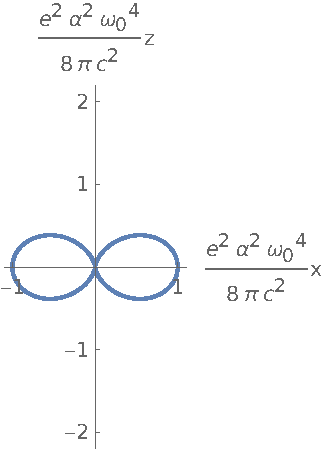
\includegraphics{3a} $\ $
				\caption{Plot of Eq.~\refeq{ans3a} in the $xz$ plane.}
				\label{3a}
			\end{figure}
		\end{minipage}%
		\hspace{0.05\linewidth}%
		\begin{minipage}{0.475\textwidth}
			\begin{figure}[H] \flushleft
				$\quad$ 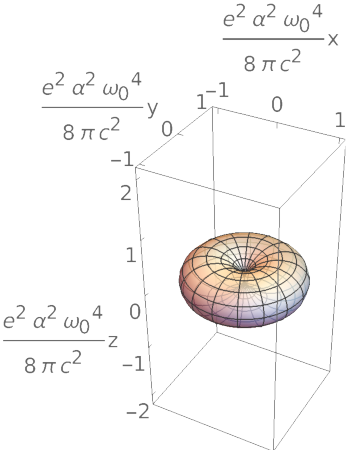
\includegraphics{3a3d}
				\caption{Three-dimensional plot of Eq.~\refeq{ans3a}.}
				\label{3a3d}
			\end{figure}
		\end{minipage}
	\end{figure}
	
	Equation~\refeq{Ptot} becomes
	\eq{
		P = \frac{2}{3} \frac{e^2}{c^3} \abs{-\alp \omgo^2 \cos \omgo t \,\xeh}^2
		= \frac{2}{3} \frac{e^2 \alp^2 \omgo^4}{c^3} \cos^2 \omgo t,
	}
	so the time-averaged total power radiated is
	\eq{
		\ev{P} = \frac{2}{3} \frac{e^2 \alp^2 \omgo^4}{c^3} \ev{\cos^2 \omgo t}
		= \ans{ \frac{e^2 \alp^2 \omgo^4}{3 c^3}. }
	}
	\vfix
}

%
%	Jackson 14.4(b)
%

\prob{}{
	The particle is moving in a circle of radius $R$ in the $xy$ plane with constant angular frequency $\omgo$.
}

\sol{
	For a charge moving counter-clockwise,
	\al{
		\vx(t) &= R \cos \omgo t \,\xqh - R \sin \omgo t \,\xwh, &
		\vv(t) &= -R \omgo \sin \omgo t \,\xqh - R \omgo \cos \omgo t \,\xwh,
	}
	\vfix
	\eq{
		\vvd(t) = -R \omgo^2 \cos \omgo t \,\xqh + R \omgo^2 \sin \omgo t \,\xwh.
	}
	This system is also azimuthally symmetric, so it is sufficient to restrict the position of the observer to the $yz$~plane.  In polar coordinates, $\nh = \sin\tht \,\xwh + \cos\tht \,\xeh$.  Then $\sin^2\Tht$ can be found by
	\eq{
		\sin^2\Tht = 1 - \cos^2\Tht
		= 1 - \frac{(\vvd \vdot \nh)^2}{\vd^2}
		= 1 - \sin^2\tht \sin^2\omgo t.
	}
	With these substitutions, Eq.~\refeq{dPdOmg} becomes
	\al{
		\dv{P}{\Omg} &= \frac{e^2}{4\pi c^2} \abs{-R \omgo^2 \cos \omgo t \,\xqh + R \omgo^2 \sin \omgo t \,\xwh}^2 (1 - \sin^2\tht \sin^2\omgo t) \\
		&= \frac{e^2 R^2 \omgo^4}{4\pi c^2} (\cos^2 \omgo t + \sin^2 \omgo t) (1 - \sin^2\tht \sin^2\omgo t)
		= \frac{e^2 R^2 \omgo^4}{4\pi c^2} (1 - \sin^2\tht \sin^2\omgo t),
	}
	giving us the time-averaged power radiated per unit solid angle:
	\aln{
		\ev{\dv{P}{\Omg}} &= \frac{e^2 R^2 \omgo^4}{4\pi c^2} (1 - \sin^2\tht \ev{\sin^2\omgo t})
		= \frac{e^2 R^2 \omgo^4}{4\pi c^2} \paren{ 1 - \frac{\sin^2\tht}{2} }
		= \frac{e^2 R^2 \omgo^4}{4\pi c^2} \paren{ 1 - \frac{1 - \cos^2\tht}{2} } \notag \\
		&= \ans{ \frac{e^2 R^2 \omgo^4}{8\pi c^2} (1 + \cos^2\tht). } \label{ans3b}
	}
	A plot of the angular distribution of the radiation in the $xz$ plane is shown in Fig.~\ref{3b}, and in three dimensions in Fig.~\ref{3b3d}.  The magnitude of the radiation on the $xy$ plane is reduced because of the particle's motion in that plane.  This is also the radiation patten for two dipoles, one on each of the $x$ and $y$ axes, oscillating out of phase $(m = \pm 1)$, as is seen in Jackson Table~{9.1} and Jackson Fig.~{9.5}.
	
	\begin{figure}[b!]
	\vspace{-6pt}
		\begin{minipage}{0.45\textwidth}
			\begin{figure}[H] \flushright
				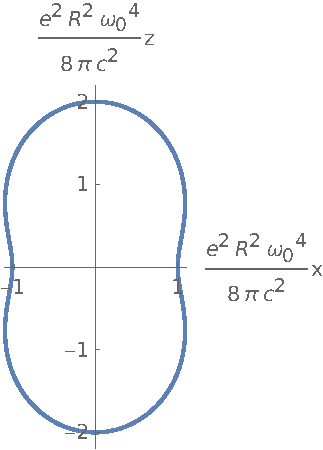
\includegraphics{3b} $\ $
				\caption{Plot of Eq.~\refeq{ans3b} in the $xz$ plane.}
				\label{3b}
			\end{figure}
		\end{minipage}%
		\hspace{0.05\linewidth}%
		\begin{minipage}{0.475\textwidth}
			\begin{figure}[H] \flushleft
				$\quad$ 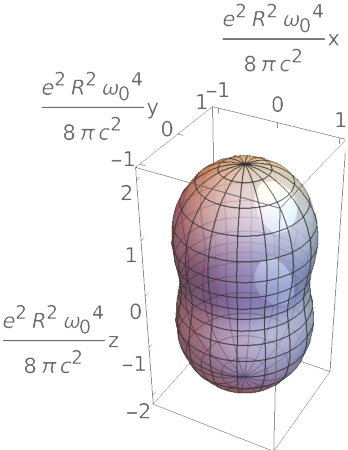
\includegraphics{3b3d}
				\caption{Three-dimensional plot of Eq.~\refeq{ans3b}.}
				\label{3b3d}
			\end{figure}
		\end{minipage}
	\end{figure}
	
	From Eq.~\refeq{Ptot}, we have
	\eq{
		P = \frac{2}{3} \frac{e^2}{c^3} \abs{-R \omgo^2 \cos \omgo t \,\xqh + R \omgo^2 \sin \omgo t \,\xwh}^2
		= \frac{2}{3} \frac{e^2 R^2 \omgo^4}{c^3} (\cos^2 \omgo t + \sin^2 \omgo t)
		= \ans{ \frac{2}{3} \frac{e^2 R^2 \omgo^4}{c^3} = \ev{P}. }
	}
	\vfix
}